\documentclass[11pt]{article}
\usepackage[utf8]{inputenc}
\usepackage[T1]{fontenc}
\usepackage{lmodern}
\usepackage[margin=1in]{geometry}
\usepackage{graphicx}
\usepackage{amsmath}
\usepackage{amssymb}
\usepackage{subcaption}
\usepackage{tikz}
\usepackage{pgfplots}
\pgfplotsset{compat=1.16}
\usepackage{xcolor}
\usepackage{listings}
\usepackage{booktabs}
\usepackage[section]{placeins}
\usepackage{cite}
\usepackage{hyperref}

\usetikzlibrary{shapes,arrows,arrows.meta,positioning,fit,backgrounds,calc}
\usepgfplotslibrary{groupplots}

% Shared figure palette and styles
\definecolor{cfrozen}{HTML}{4C72B0}
\definecolor{ctrain}{HTML}{DD8452}
\definecolor{cdata}{HTML}{55A868}
\definecolor{ccond}{HTML}{8172B3}
\definecolor{cmetric}{HTML}{C44E52}
\definecolor{cgray}{HTML}{8C8C8C}
\tikzset{
  >=Stealth,
  blk/.style={draw=#1!70!black, fill=#1!15, rounded corners=2pt, align=center,
              minimum height=0.8cm, inner sep=4pt, font=\small},
  blk/.default=cgray,
  region/.style={draw=#1!60, fill=#1!5, rounded corners=6pt, dashed, inner sep=8pt},
  lbl/.style={font=\footnotesize, inner sep=1pt},
  flow/.style={->, thick, draw=black!75},
}
\pgfplotsset{
  every axis/.append style={font=\small, grid=major, grid style={gray!25},
    tick label style={font=\footnotesize}, label style={font=\small},
    legend style={font=\footnotesize, draw=gray!50}},
  cycle list={{cfrozen, mark=*, thick},{ctrain, mark=square*, thick},
              {cdata, mark=triangle*, thick},{cmetric, mark=diamond*, thick}},
}

\lstset{basicstyle=\ttfamily\small, columns=fullflexible, breaklines=true}

\title{Text-to-Image Generation with Diffusion Models:\\
{\large Part 3: Evaluation Metrics \& Ablation Studies}}
\author{Person C}
\date{\today}

\begin{document}

\maketitle

\begin{abstract}
This report details the evaluation methodology and 8 ablation studies (A01--A08) for text-to-image generation. We use three evaluation metrics: FID (Fr\'echet Inception Distance) for image quality, KID (Kernel Inception Distance) for unbiased comparison, and CLIP Score for prompt-image alignment. We conduct systematic ablations on LoRA fine-tuning, guidance scale, sampling steps, schedulers, LoRA rank, training duration, negative prompts, and base architecture. LoRA rank 32 gives the best FID overall (75.26); among inference settings, guidance scale 5.0 (FID 78.96) and the DDIM scheduler at 30 steps (FID 80.46) perform best. Our LoRA-tuned SD v1.5 outperforms zero-shot SDXL, although the SDXL result requires verification (Section~\ref{sec:a08}).
\end{abstract}

\section{Introduction}

Evaluating generative models requires metrics beyond visual inspection. We employ three complementary metrics:

\begin{enumerate}
    \item \textbf{FID}~\cite{heusel2017gans}: Statistical similarity between generated and real images
    \item \textbf{KID}~\cite{binkowski2018demystifying}: Unbiased alternative to FID, better suited to small sample sizes
    \item \textbf{CLIP Score}~\cite{hessel2021clipscore}: Semantic alignment between prompt and image
\end{enumerate}

We run 8 ablation studies (A01--A08) to identify good settings.

\section{Evaluation Metrics}

\subsection{FID (Fr\'echet Inception Distance)}

FID measures the distance between Gaussian fits to real and generated images in InceptionV3 feature space:

\begin{equation}
\text{FID} = \|\mathbf{m}_r - \mathbf{m}_g\|_2^2 + \text{Tr}\left(\Sigma_r + \Sigma_g - 2(\Sigma_r \Sigma_g)^{1/2}\right)
\end{equation}

where:
\begin{itemize}
    \item $\mathbf{m}_r, \mathbf{m}_g$: mean activations (real vs.\ generated)
    \item $\Sigma_r, \Sigma_g$: covariance matrices
\end{itemize}

\textbf{Range}: $[0, \infty)$, where 0 means identical feature statistics.
\textbf{Lower is better}.

\subsection{KID (Kernel Inception Distance)}

KID is the squared Maximum Mean Discrepancy (MMD) between Inception features of real and generated images, using a cubic polynomial kernel:

\begin{equation}
\text{KID} = \text{MMD}^2(\{I_r\}, \{I_g\})
\end{equation}

Advantages over FID:
\begin{itemize}
    \item Unbiased estimator
    \item More reliable with small sample sizes (we use 1,000 generated images)
\end{itemize}

\subsection{CLIP Score}

CLIP Score~\cite{hessel2021clipscore} measures semantic alignment using CLIP~\cite{radford2021learning}:

\begin{equation}
\text{CLIP Score} = 100 \times \max\left(\cos(\mathbf{v}_i, \mathbf{v}_t), 0\right)
\end{equation}

where:
\begin{itemize}
    \item $\mathbf{v}_i$: CLIP image embedding (ViT-B/32)
    \item $\mathbf{v}_t$: CLIP text embedding
    \item $\cos(\cdot)$: cosine similarity
\end{itemize}

\textbf{Range}: $[0, 100]$; higher means better alignment (typical values for well-matched pairs are around 30).
\textbf{Higher is better}.

\section{Evaluation Protocol}

\subsection{Fixed Test Set}

All ablations use:
\begin{itemize}
    \item \textbf{200 fixed prompts} from a curated set
    \item \textbf{5 seeds} per prompt: [0, 1, 2, 3, 4]
    \item \textbf{Total generated images}: $200 \times 5 = 1{,}000$
    \item \textbf{Real images}: 6,149 from the test split
\end{itemize}

Using fixed prompts and seeds ensures fair comparison across ablations. Note that FID is biased upward at small sample sizes, so our absolute FID values (computed from 1,000 generated images) are not directly comparable to published numbers; only relative comparisons within this report are meaningful. Unless stated otherwise, the default configuration is LoRA rank 16 (final checkpoint), guidance scale 7.5, DPM-Solver++ with 30 steps, and no negative prompt. Figure~\ref{fig:eval_pipeline} summarizes the protocol.

\begin{figure}[!htbp]
\centering
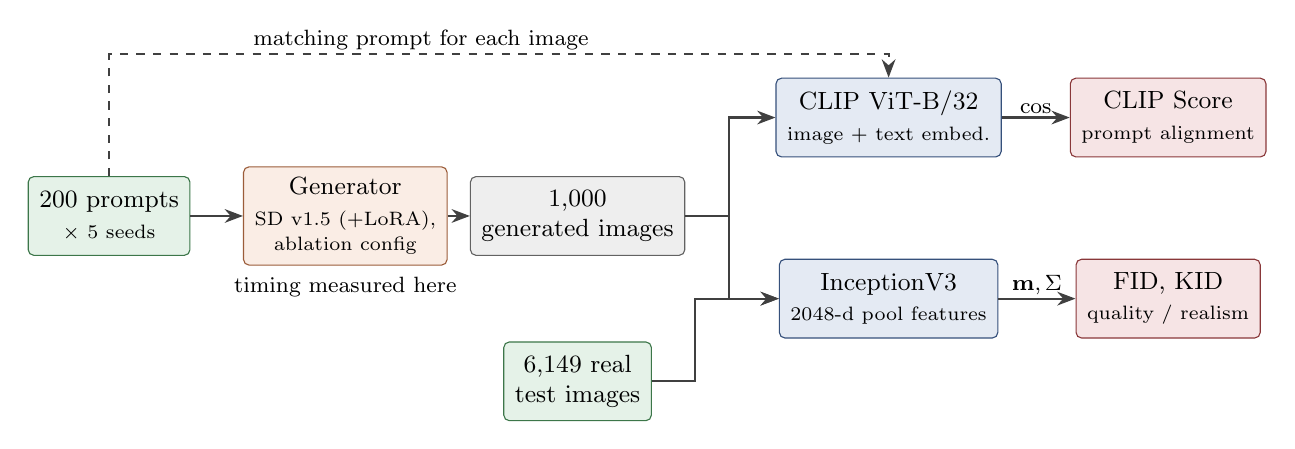
\begin{tikzpicture}[eb/.style={blk=#1, minimum height=1.0cm}]
  \node[eb=cdata] (pr) at (0,0) {200 prompts\\{\scriptsize $\times$ 5 seeds}};
  \node[eb=ctrain] (gen) at (3.0,0) {Generator\\{\scriptsize SD v1.5 (+LoRA),}\\[-2pt]{\scriptsize ablation config}};
  \node[eb] (gi) at (5.95,0) {1,000\\generated images};
  \node[eb=cdata] (ri) at (5.95,-2.1) {6,149 real\\test images};
  \node[eb=cfrozen] (inc) at (9.9,-1.05) {InceptionV3\\{\scriptsize 2048-d pool features}};
  \node[eb=cfrozen] (clip) at (9.9,1.25) {CLIP ViT-B/32\\{\scriptsize image + text embed.}};
  \node[eb=cmetric] (fk) at (13.45,-1.05) {FID, KID\\{\scriptsize quality / realism}};
  \node[eb=cmetric] (cs) at (13.45,1.25) {CLIP Score\\{\scriptsize prompt alignment}};
  \draw[flow] (pr) -- (gen);
  \draw[flow] (gen) -- (gi);
  \draw[flow] (gi.east) -- ++(0.55,0) |- (inc.west);
  \draw[flow] (ri.east) -- ++(0.55,0) |- (inc.west);
  \draw[flow] (gi.east) -- ++(0.55,0) |- (clip.west);
  \draw[flow, dashed] (pr.north) -- ++(0,1.55) -| node[lbl, pos=0.2, above] {matching prompt for each image} (clip.north);
  \draw[flow] (inc) -- node[lbl, above] {$\mathbf{m},\Sigma$} (fk);
  \draw[flow] (clip) -- node[lbl, above] {$\cos$} (cs);
  \node[lbl, below=3pt of gen] {timing measured here};
\end{tikzpicture}
\caption{Evaluation protocol used for every ablation. Generated images are compared with the real test split in Inception feature space (FID, KID) and with their own prompts in CLIP space (CLIP Score).}
\label{fig:eval_pipeline}
\end{figure}

\subsection{Metric Computation}

\begin{lstlisting}[language=Python, caption=Evaluation pipeline]
# 1. Generate 1,000 images (200 prompts x 5 seeds)
pairs = [(p, s) for p in prompts for s in range(5)]
images = [model.generate(prompt=p, seed=s) for p, s in pairs]

# 2. Compute FID/KID against the 6,149 real test images
fid, kid = compute_fid_kid(images, real_images)

# 3. Compute CLIP Score (each image vs. its own prompt)
clip_scores = [clip_model.score(img, p)
               for img, (p, _) in zip(images, pairs)]
clip_avg = np.mean(clip_scores)

# 4. Measure timing
time_per_image = total_time / len(images)
\end{lstlisting}

\section{Ablation Study Results}

Each ablation changes one factor relative to the default configuration (Figure~\ref{fig:ablation_map}).

\begin{figure}[!htbp]
\centering
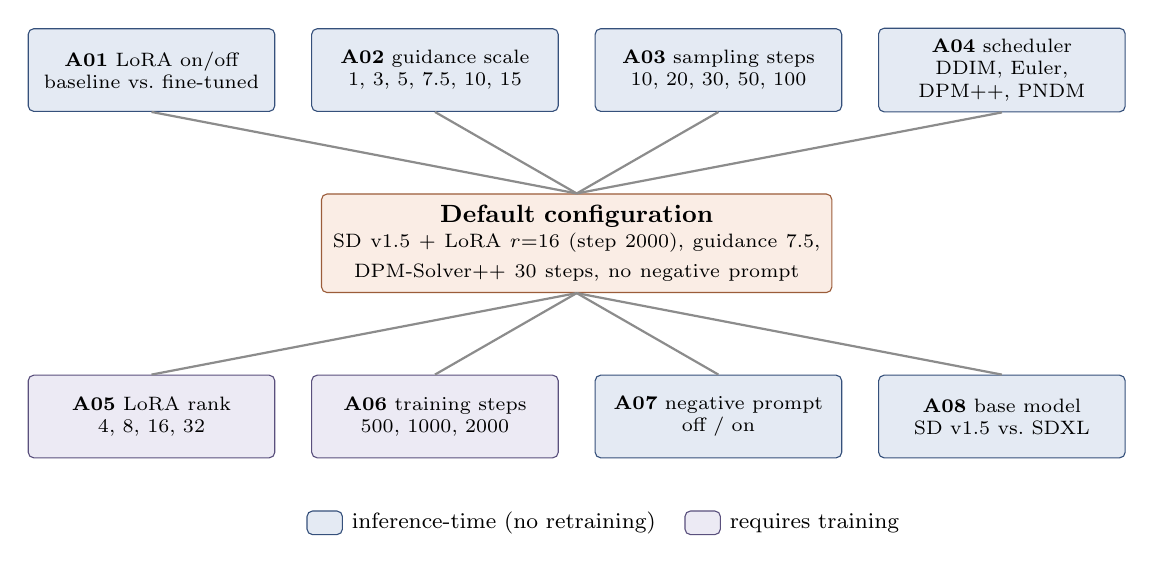
\begin{tikzpicture}[ab/.style={blk=#1, text width=2.85cm, minimum height=1.05cm, font=\scriptsize}]
  \node[blk=ctrain, text width=6.2cm, font=\small] (def) at (0,0)
     {\textbf{Default configuration}\\[1pt]{\scriptsize SD v1.5 + LoRA $r{=}16$ (step 2000), guidance 7.5,\\DPM-Solver++ 30 steps, no negative prompt}};
  \node[ab=cfrozen] (a1) at (-5.4,2.2) {\textbf{A01} LoRA on/off\\baseline vs.\ fine-tuned};
  \node[ab=cfrozen] (a2) at (-1.8,2.2) {\textbf{A02} guidance scale\\1, 3, 5, 7.5, 10, 15};
  \node[ab=cfrozen] (a3) at (1.8,2.2)  {\textbf{A03} sampling steps\\10, 20, 30, 50, 100};
  \node[ab=cfrozen] (a4) at (5.4,2.2)  {\textbf{A04} scheduler\\DDIM, Euler, DPM++, PNDM};
  \node[ab=ccond] (a5) at (-5.4,-2.2) {\textbf{A05} LoRA rank\\4, 8, 16, 32};
  \node[ab=ccond] (a6) at (-1.8,-2.2) {\textbf{A06} training steps\\500, 1000, 2000};
  \node[ab=cfrozen] (a7) at (1.8,-2.2) {\textbf{A07} negative prompt\\off / on};
  \node[ab=cfrozen] (a8) at (5.4,-2.2) {\textbf{A08} base model\\SD v1.5 vs.\ SDXL};
  \foreach \n in {a1,a2,a3,a4} \draw[thick, cgray] (def.north) -- (\n.south);
  \foreach \n in {a5,a6,a7,a8} \draw[thick, cgray] (def.south) -- (\n.north);
  \node[blk=cfrozen, minimum width=0.45cm, minimum height=0.3cm] (l1) at (-3.2,-3.55) {};
  \node[lbl, right=2pt of l1] {inference-time (no retraining)};
  \node[blk=ccond, minimum width=0.45cm, minimum height=0.3cm] (l2) at (1.6,-3.55) {};
  \node[lbl, right=2pt of l2] {requires training};
\end{tikzpicture}
\caption{Overview of the eight one-factor-at-a-time ablations around the default configuration.}
\label{fig:ablation_map}
\end{figure}

\subsection{A01: Baseline vs LoRA}

\begin{table}[!htbp]
\centering
\caption{A01: Does LoRA fine-tuning help?}
\begin{tabular}{lrrr}
\toprule
Model & FID $\downarrow$ & KID $\downarrow$ & CLIP $\uparrow$ \\
\midrule
SD v1.5 Baseline & 87.25 & 0.0357 & 31.34 \\
SD v1.5 + LoRA & 85.49 & 0.0310 & 31.38 \\
Change & $-2.0\%$ & $-13.2\%$ & $+0.1\%$ \\
\bottomrule
\end{tabular}
\end{table}

\textbf{Finding}: The modest FID improvement (2\%) reflects that SD v1.5 already has substantial flower knowledge. KID shows a larger improvement (13\%), suggesting better distribution alignment, while CLIP Score is essentially unchanged (Figure~\ref{fig:a01}).

\begin{figure}[!htbp]
\centering
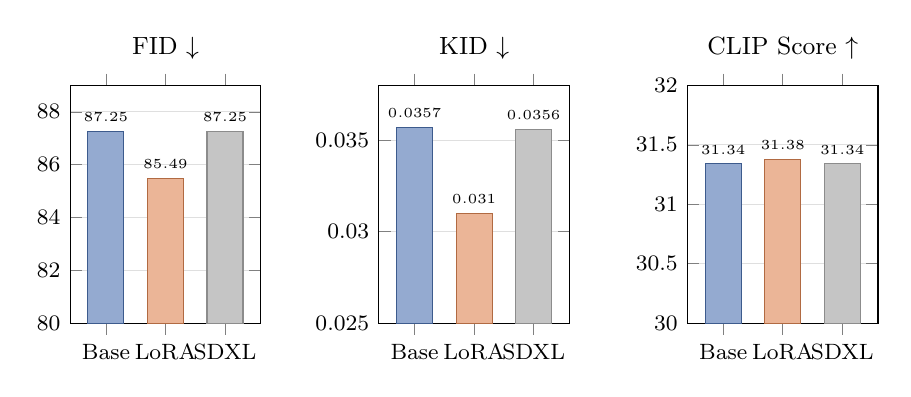
\begin{tikzpicture}
\begin{groupplot}[group style={group size=3 by 1, horizontal sep=1.5cm},
    width=0.33\linewidth, height=4.6cm, ybar, /pgf/bar width=13pt, /pgf/bar shift=0pt,
    symbolic x coords={Base,LoRA,SDXL}, xtick={Base,LoRA,SDXL}, xmajorgrids=false, enlarge x limits=0.3,
    nodes near coords, every node near coord/.append style={font=\tiny}]
\nextgroupplot[title={\small FID $\downarrow$}, ymin=80, ymax=89]
\addplot[fill=cfrozen!60, draw=cfrozen!80!black] coordinates {(Base,87.25)};
\addplot[fill=ctrain!60, draw=ctrain!80!black] coordinates {(LoRA,85.49)};
\addplot[fill=cgray!50, draw=cgray] coordinates {(SDXL,87.25)};
\nextgroupplot[title={\small KID $\downarrow$}, ymin=0.025, ymax=0.038, yticklabel style={/pgf/number format/fixed, /pgf/number format/precision=3}, scaled y ticks=false,
    every node near coord/.append style={/pgf/number format/fixed, /pgf/number format/precision=4}]
\addplot[fill=cfrozen!60, draw=cfrozen!80!black] coordinates {(Base,0.0357)};
\addplot[fill=ctrain!60, draw=ctrain!80!black] coordinates {(LoRA,0.0310)};
\addplot[fill=cgray!50, draw=cgray] coordinates {(SDXL,0.0356)};
\nextgroupplot[title={\small CLIP Score $\uparrow$}, ymin=30, ymax=32]
\addplot[fill=cfrozen!60, draw=cfrozen!80!black] coordinates {(Base,31.34)};
\addplot[fill=ctrain!60, draw=ctrain!80!black] coordinates {(LoRA,31.38)};
\addplot[fill=cgray!50, draw=cgray] coordinates {(SDXL,31.34)};
\end{groupplot}
\end{tikzpicture}
\caption{A01 and A08: zero-shot SD v1.5 (Base), LoRA-tuned SD v1.5, and zero-shot SDXL. Note the truncated y-axes; the SDXL values require verification (Section~\ref{sec:a08}).}
\label{fig:a01}
\end{figure}

\subsection{A02: Guidance Scale}

\begin{table}[!htbp]
\centering
\caption{A02: Classifier-free guidance scale (1 to 15)}
\begin{tabular}{lrrrr}
\toprule
Scale & FID & KID & CLIP & Time \\
\midrule
1.0 & 122.86 & 0.0599 & 26.73 & 12.46s \\
3.0 & 80.68 & 0.0336 & 31.04 & 12.45s \\
5.0 & 78.96 & 0.0294 & 31.48 & 12.43s \\
7.5 & 85.49 & 0.0308 & 31.38 & 12.47s \\
10.0 & 92.57 & 0.0335 & 31.12 & 12.63s \\
15.0 & 113.04 & 0.0444 & 30.38 & 12.46s \\
\bottomrule
\end{tabular}
\end{table}

\textbf{Finding}: The optimal classifier-free guidance~\cite{ho2022classifier} scale is \textbf{5.0} (FID 78.96), which also gives the best KID and CLIP Score. Too low (1.0, i.e.\ no guidance) gives poor prompt adherence and quality; too high (15.0) causes over-saturation, artifacts and reduced diversity.

\begin{figure}[!htbp]
\centering
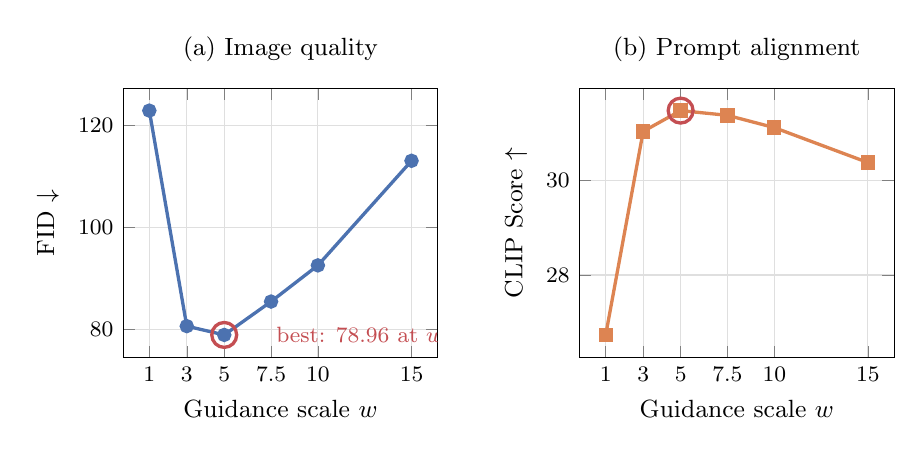
\begin{tikzpicture}
\begin{groupplot}[group style={group size=2 by 1, horizontal sep=1.8cm},
    width=0.46\linewidth, height=5cm, xlabel={Guidance scale $w$}, xtick={1,3,5,7.5,10,15}]
\nextgroupplot[ylabel={FID $\downarrow$}, title={\small (a) Image quality}]
\addplot+[cfrozen, mark=*, very thick] coordinates {(1,122.86) (3,80.68) (5,78.96) (7.5,85.49) (10,92.57) (15,113.04)};
\node[circle, draw=cmetric, very thick, minimum size=9pt, inner sep=0pt] at (axis cs:5,78.96) {};
\node[lbl, anchor=west, text=cmetric] at (axis cs:7.6,79) {best: 78.96 at $w{=}5$};
\nextgroupplot[ylabel={CLIP Score $\uparrow$}, title={\small (b) Prompt alignment}]
\addplot+[ctrain, mark=square*, very thick] coordinates {(1,26.73) (3,31.04) (5,31.48) (7.5,31.38) (10,31.12) (15,30.38)};
\node[circle, draw=cmetric, very thick, minimum size=9pt, inner sep=0pt] at (axis cs:5,31.48) {};
\end{groupplot}
\end{tikzpicture}
\caption{A02: effect of classifier-free guidance scale. Both FID and CLIP Score are optimal at $w=5.0$ (circled); the default $w=7.5$ is slightly too strong for this domain.}
\label{fig:a02}
\end{figure}

\subsection{A03: Sampling Steps}

\begin{table}[!htbp]
\centering
\caption{A03: Number of sampling steps (DPM-Solver++)}
\begin{tabular}{lrrrr}
\toprule
Steps & FID & KID & CLIP & Time \\
\midrule
10 & 83.03 & 0.0307 & 31.42 & 4.53s \\
20 & 82.59 & 0.0297 & 31.45 & 8.56s \\
30 & 85.49 & 0.0308 & 31.38 & 12.87s \\
50 & 86.99 & 0.0313 & 31.35 & 20.76s \\
100 & 88.36 & 0.0318 & 31.29 & 40.61s \\
\bottomrule
\end{tabular}
\end{table}

\textbf{Finding}: Best at \textbf{20 steps (FID 82.59)}. Beyond 20 steps, FID worsens slightly while time grows linearly. For production: 10 steps (fast) or 20 steps (quality). Figure~\ref{fig:a03} shows the quality--speed trade-off.

\begin{figure}[!htbp]
\centering
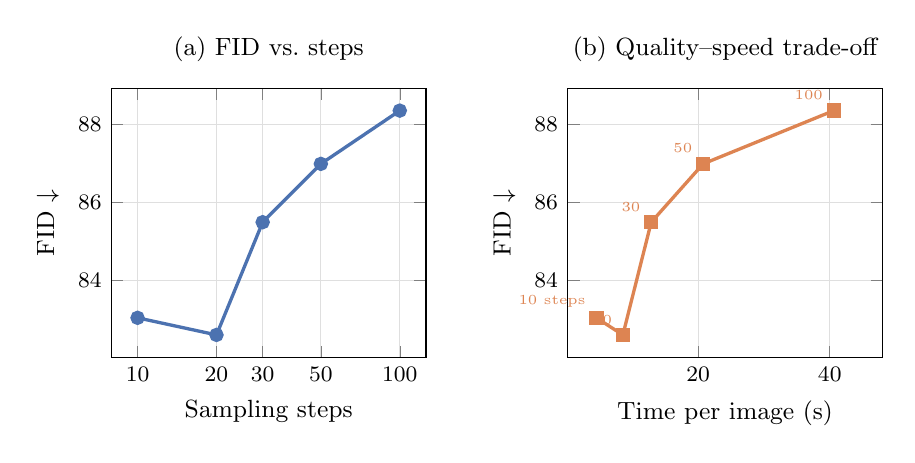
\begin{tikzpicture}
\begin{groupplot}[group style={group size=2 by 1, horizontal sep=1.8cm}, width=0.46\linewidth, height=5cm]
\nextgroupplot[xmode=log, log basis x=10, xtick={10,20,30,50,100}, xticklabels={10,20,30,50,100},
               xlabel={Sampling steps}, ylabel={FID $\downarrow$}, title={\small (a) FID vs.\ steps}]
\addplot+[cfrozen, mark=*, very thick] coordinates {(10,83.03) (20,82.59) (30,85.49) (50,86.99) (100,88.36)};
\nextgroupplot[xlabel={Time per image (s)}, ylabel={FID $\downarrow$}, title={\small (b) Quality--speed trade-off},
               xmax=48, nodes near coords, point meta=explicit symbolic,
               every node near coord/.append style={font=\tiny, anchor=south east}]
\addplot+[ctrain, mark=square*, very thick] coordinates {(4.53,83.03)[10 steps] (8.56,82.59)[20] (12.87,85.49)[30] (20.76,86.99)[50] (40.61,88.36)[100]};
\end{groupplot}
\end{tikzpicture}
\caption{A03: sampling steps with DPM-Solver++. Time grows linearly with steps, while FID is best at 10--20 steps.}
\label{fig:a03}
\end{figure}

\subsection{A04: Scheduler Comparison}

\begin{table}[!htbp]
\centering
\caption{A04: Denoising scheduler (4 schedulers $\times$ 2 step counts)}
\begin{tabular}{lrrrr}
\toprule
Scheduler & Steps & FID & KID & Time \\
\midrule
DDIM~\cite{song2021denoising} & 10 & 97.08 & 0.0482 & 4.47s \\
DDIM & 30 & 80.46 & 0.0325 & 13.16s \\
Euler~\cite{karras2022elucidating} & 10 & 87.30 & 0.0324 & 4.56s \\
Euler & 30 & 82.26 & 0.0292 & 12.78s \\
DPM-Solver++~\cite{lu2022dpmsolverpp} & 10 & 83.03 & 0.0307 & 4.52s \\
DPM-Solver++ & 30 & 85.49 & 0.0308 & 12.79s \\
PNDM~\cite{liu2022pseudo} & 10 & 93.62 & 0.0455 & 4.72s \\
PNDM & 30 & 85.96 & 0.0338 & 12.64s \\
\bottomrule
\end{tabular}
\end{table}

\textbf{Finding}: \textbf{DDIM at 30 steps achieves the best scheduler FID (80.46)}, while Euler at 30 steps is close in FID (82.26) and has the best KID (0.0292). PNDM underperforms. At 10 steps, DPM-Solver++ is best (83.03).

\begin{figure}[!htbp]
\centering
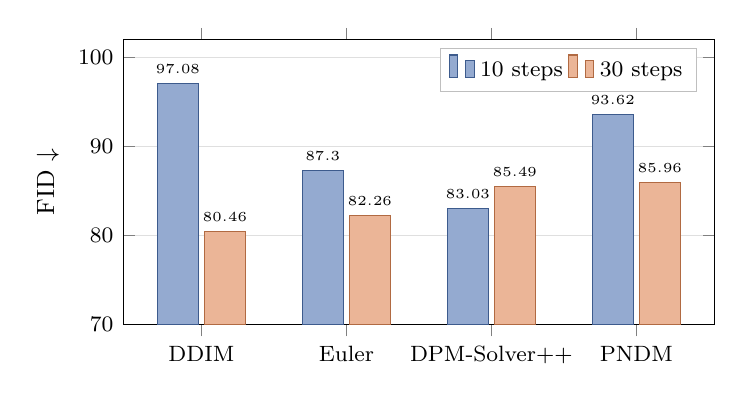
\begin{tikzpicture}
\begin{axis}[ybar, width=0.75\linewidth, height=5.2cm, bar width=15pt, ymin=70, ymax=102,
             symbolic x coords={DDIM,Euler,DPM-Solver++,PNDM}, xtick=data, xmajorgrids=false,
             ylabel={FID $\downarrow$}, enlarge x limits=0.18, legend pos=north east, legend columns=2,
             nodes near coords, every node near coord/.append style={font=\tiny}]
\addplot[fill=cfrozen!60, draw=cfrozen!80!black] coordinates {(DDIM,97.08) (Euler,87.30) (DPM-Solver++,83.03) (PNDM,93.62)};
\addplot[fill=ctrain!60, draw=ctrain!80!black] coordinates {(DDIM,80.46) (Euler,82.26) (DPM-Solver++,85.49) (PNDM,85.96)};
\legend{10 steps, 30 steps}
\end{axis}
\end{tikzpicture}
\caption{A04: FID for each scheduler at 10 and 30 sampling steps. DDIM benefits most from more steps; DPM-Solver++ is the only scheduler that is better at 10 steps.}
\label{fig:a04}
\end{figure}

\subsection{A05: LoRA Rank}

\begin{table}[!htbp]
\centering
\caption{A05: LoRA capacity (complete results)}
\begin{tabular}{lrrr}
\toprule
Rank & Params & FID & KID \\
\midrule
4 & 0.80M & 82.03 & 0.0309 \\
8 & 1.59M & 79.16 & 0.0302 \\
16 & 3.19M & 85.49 & 0.0311 \\
32 & 6.38M & 75.26 & 0.0259 \\
\bottomrule
\end{tabular}
\end{table}

\textbf{Major Finding}: \textbf{Rank 32 achieves FID 75.26, the best result across all ablations}. The relationship between rank and FID is non-monotonic: rank 8 (FID 79.16) outperforms rank 16 (FID 85.49), the rank used for our main model. Since each rank was trained once, part of this variation may be due to training randomness. For maximum quality, rank 32 is recommended despite higher memory use.

\begin{figure}[!htbp]
\centering
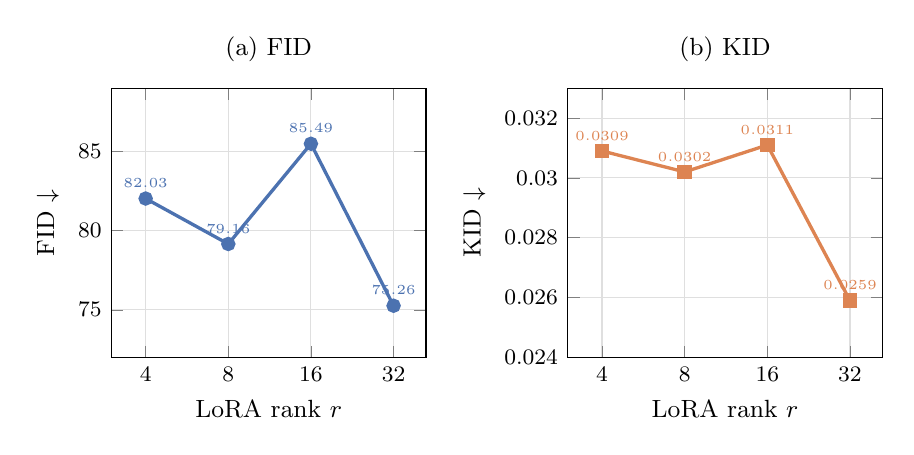
\begin{tikzpicture}
\begin{groupplot}[group style={group size=2 by 1, horizontal sep=1.8cm}, width=0.46\linewidth, height=5cm,
                  xmode=log, log basis x=2, xtick={4,8,16,32}, xticklabels={4,8,16,32}, xlabel={LoRA rank $r$},
                  xmin=3, xmax=42,
                  nodes near coords, every node near coord/.append style={font=\tiny, anchor=south}]
\nextgroupplot[ylabel={FID $\downarrow$}, title={\small (a) FID}, ymin=72, ymax=89]
\addplot+[cfrozen, mark=*, very thick] coordinates {(4,82.03) (8,79.16) (16,85.49) (32,75.26)};
\nextgroupplot[ylabel={KID $\downarrow$}, title={\small (b) KID}, ymin=0.024, ymax=0.033,
               scaled y ticks=false, yticklabel style={/pgf/number format/fixed, /pgf/number format/precision=3},
               every node near coord/.append style={/pgf/number format/fixed, /pgf/number format/precision=4}]
\addplot+[ctrain, mark=square*, very thick] coordinates {(4,0.0309) (8,0.0302) (16,0.0311) (32,0.0259)};
\end{groupplot}
\end{tikzpicture}
\caption{A05: FID and KID versus LoRA rank (log scale). Both metrics agree that rank 32 is best and rank 16 worst.}
\label{fig:a05}
\end{figure}

\subsection{A06: Training Steps Impact}

\begin{table}[!htbp]
\centering
\caption{A06: Training duration (checkpoints from the same rank-16 run)}
\begin{tabular}{lrrr}
\toprule
Step & Checkpoint & FID & KID \\
\midrule
500 & Early & 79.89 & 0.0312 \\
1000 & Mid & 82.16 & 0.0304 \\
2000 & Final & 85.49 & 0.0310 \\
\bottomrule
\end{tabular}
\end{table}

\textbf{Finding}: The earliest checkpoint (step 500) achieves the \textbf{best FID (79.89)}, although KID is lowest at step 1000 and the KID differences are small. This suggests some overfitting or distribution shift after 500 steps on this small training set (1,020 images).

\begin{figure}[!htbp]
\centering
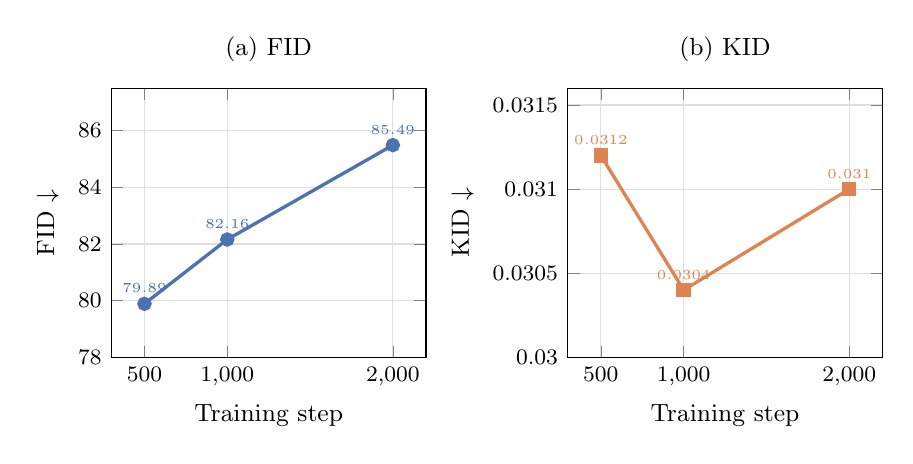
\begin{tikzpicture}
\begin{groupplot}[group style={group size=2 by 1, horizontal sep=1.8cm}, width=0.46\linewidth, height=5cm,
                  xtick={500,1000,2000}, xlabel={Training step}, xmin=300, xmax=2200,
                  nodes near coords, every node near coord/.append style={font=\tiny, anchor=south}]
\nextgroupplot[ylabel={FID $\downarrow$}, title={\small (a) FID}, ymin=78, ymax=87.5]
\addplot+[cfrozen, mark=*, very thick] coordinates {(500,79.89) (1000,82.16) (2000,85.49)};
\nextgroupplot[ylabel={KID $\downarrow$}, title={\small (b) KID}, ymin=0.0300, ymax=0.0316,
               scaled y ticks=false, yticklabel style={/pgf/number format/fixed, /pgf/number format/precision=4},
               every node near coord/.append style={/pgf/number format/fixed, /pgf/number format/precision=4}]
\addplot+[ctrain, mark=square*, very thick] coordinates {(500,0.0312) (1000,0.0304) (2000,0.0310)};
\end{groupplot}
\end{tikzpicture}
\caption{A06: checkpoints from the same rank-16 run. FID rises steadily with training; KID varies within a narrow range (note the y-axis scale).}
\label{fig:a06}
\end{figure}

\subsection{A07: Negative Prompts}

\begin{table}[!htbp]
\centering
\caption{A07: Negative prompt effect}
\begin{tabular}{lrrr}
\toprule
Setting & FID & KID & CLIP \\
\midrule
No negative & 85.49 & 0.0308 & 31.38 \\
With negative & 86.06 & 0.0325 & 30.94 \\
Change & $+0.7\%$ & $+5.5\%$ & $-1.4\%$ \\
\bottomrule
\end{tabular}
\end{table}

\textbf{Finding}: Negative prompts slightly \textbf{hurt} all three metrics. The generic negative prompt (``blurry, low quality\ldots'') appears too broad for flowers and may reduce diversity (e.g., suppressing soft-focus backgrounds common in the real images).

\subsection{A08: Architecture Comparison}
\label{sec:a08}

\begin{table}[!htbp]
\centering
\caption{A08: Model architecture}
\begin{tabular}{lrrr}
\toprule
Model & FID & KID & CLIP \\
\midrule
SD v1.5 Baseline & 87.25 & 0.0357 & 31.34 \\
SD v1.5 + LoRA & 85.49 & 0.0310 & 31.38 \\
SDXL~\cite{podell2023sdxl} Zero-shot & 87.25 & 0.0356 & 31.34 \\
\bottomrule
\end{tabular}
\end{table}

\textbf{Finding}: Our LoRA-tuned SD v1.5 achieves better FID and KID than zero-shot SDXL on this domain. \textbf{Caveat}: the SDXL results match the SD v1.5 baseline almost exactly on all three metrics, which is very unlikely for a different model and may indicate that the SD v1.5 pipeline was evaluated in place of SDXL. This result should be re-run (at SDXL's native $1024 \times 1024$ resolution, resized for evaluation) before drawing conclusions.
% TODO(verify): confirm the SDXL checkpoint was actually loaded in this run.

\section{Ablation Summary Table}

\begin{table}[!htbp]
\centering
\caption{All ablations summary (complete results)}
\begin{tabular}{llrl}
\toprule
Ablation & Best Value & Best FID & Notes \\
\midrule
A01 & LoRA & 85.49 & vs.\ baseline 87.25 \\
A02 & Guidance = 5.0 & 78.96 & Sweet spot \\
A03 & Steps = 20 & 82.59 & Optimal middle ground \\
A04 & DDIM, 30 steps & 80.46 & Scheduler + steps \\
A05 & Rank = 32 & 75.26 & \textbf{Best overall} \\
A06 & Step = 500 & 79.89 & Early stopping helps \\
A07 & No negative & 85.49 & Negative prompt hurts \\
A08 & SD v1.5 + LoRA & 85.49 & Beats SDXL (to verify) \\
\bottomrule
\end{tabular}
\end{table}

\begin{figure}[!htbp]
\centering
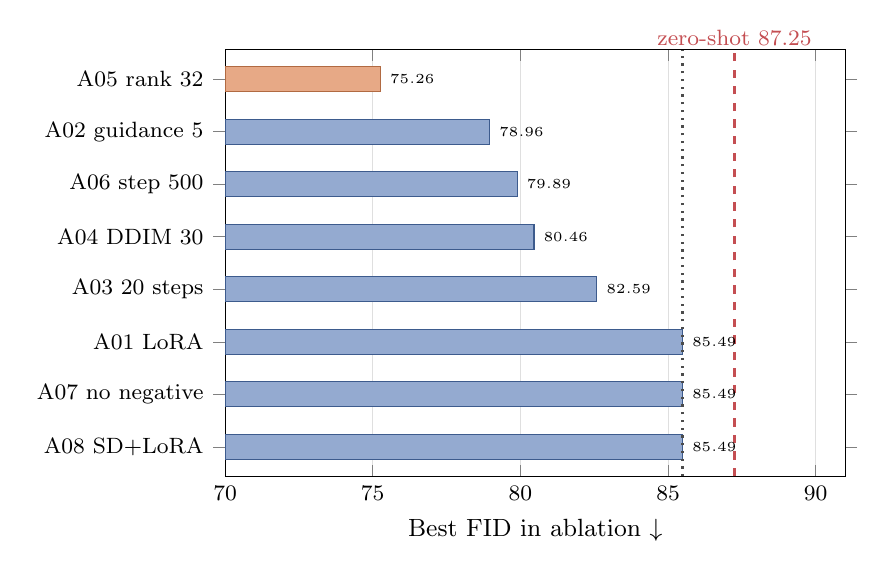
\begin{tikzpicture}
\begin{axis}[xbar, /pgf/bar shift=0pt, clip=false, width=0.78\linewidth, height=7cm, bar width=9pt, xmin=70, xmax=91,
             xlabel={Best FID in ablation $\downarrow$},
             symbolic y coords={A08 SD+LoRA,A07 no negative,A01 LoRA,A03 20 steps,A04 DDIM 30,A06 step 500,A02 guidance 5,A05 rank 32},
             ytick={A08 SD+LoRA,A07 no negative,A01 LoRA,A03 20 steps,A04 DDIM 30,A06 step 500,A02 guidance 5,A05 rank 32},
             ymajorgrids=false, enlarge y limits=0.08,
             nodes near coords, every node near coord/.append style={font=\tiny}]
\addplot[fill=cfrozen!60, draw=cfrozen!80!black] coordinates {(85.49,A08 SD+LoRA) (85.49,A07 no negative) (85.49,A01 LoRA) (82.59,A03 20 steps) (80.46,A04 DDIM 30) (79.89,A06 step 500) (78.96,A02 guidance 5)};
\addplot[fill=ctrain!70, draw=ctrain!80!black, bar shift=0pt] coordinates {(75.26,A05 rank 32)};
\draw[dashed, thick, cmetric] ({axis cs:87.25,A01 LoRA}|-{rel axis cs:0,0}) -- ({axis cs:87.25,A01 LoRA}|-{rel axis cs:0,1})
      node[lbl, anchor=south, text=cmetric] {zero-shot 87.25};
\draw[dotted, thick, black!70] ({axis cs:85.49,A01 LoRA}|-{rel axis cs:0,0}) -- ({axis cs:85.49,A01 LoRA}|-{rel axis cs:0,1});
\end{axis}
\end{tikzpicture}
\caption{Best FID achieved in each ablation, sorted. Dashed red line: zero-shot SD v1.5 baseline; dotted line: default LoRA configuration (85.49). Rank 32 (orange) gives the largest gain.}
\label{fig:summary}
\end{figure}

\section{Key Insights}

\subsection{Recommended Generation Settings}

Each ablation varies one factor from the default configuration. The settings below combine the individual winners; their combination has not been evaluated jointly and the effects may not be additive.

\textbf{Recommended starting point for flowers:}
\begin{itemize}
    \item Model: SD v1.5 + LoRA \textbf{rank 32}
    \item Guidance: \textbf{5.0}
    \item Scheduler: \textbf{DDIM}
    \item Steps: \textbf{30} with DDIM (best quality); with DPM-Solver++, 20 (balanced) or 10 (speed)
    \item Checkpoint: an \textbf{early checkpoint} (step 500 was best for rank 16; not yet tested for rank 32)
    \item No negative prompt
\end{itemize}

\textbf{Best FID measured}: \textbf{75.26 (A05, rank 32)}\\
\textbf{Second best}: 78.96 (A02, guidance 5.0 with rank 16)

\subsection{Surprising Findings}

\begin{enumerate}
    \item \textbf{Rank 32 beats rank 16}: Rank 32 (6.4M parameters) achieves FID 75.26 vs.\ FID 85.49 for rank 16 (3.2M), but the trend is not monotonic (see next item).
    \item \textbf{Rank 8 beats rank 16}: Rank 8 (1.6M parameters) achieves FID 79.16, clearly better than our main rank-16 model (85.49).
    \item \textbf{Step 500 beats step 2000}: Training longer worsens FID (500: 79.89 vs.\ 2000: 85.49), suggesting overfitting to the small training set.
    \item \textbf{Negative prompts hurt}: Generic negatives reduce quality for this specialized domain (FID 85.49 $\to$ 86.06).
    \item \textbf{SDXL zero-shot matches the SD v1.5 baseline}: The larger SDXL model reports the same FID as zero-shot SD v1.5 (87.25); this needs to be verified (Section~\ref{sec:a08}).
\end{enumerate}

\section{Conclusion}

We have conducted a comprehensive evaluation of text-to-image generation on Oxford-102 Flowers. Key contributions:

\begin{itemize}
    \item Established an evaluation protocol with 3 complementary metrics
    \item Ran 8 ablation studies covering fine-tuning, inference settings, LoRA rank, training duration and base architecture
    \item Demonstrated LoRA efficiency (main model: 3.2M trainable parameters, 0.37\% of the U-Net)
    \item Achieved a best FID of 75.26 (LoRA rank 32), with guidance 5.0 giving the best inference-time improvement (FID 78.96)
\end{itemize}

The ablation results provide actionable guidance for practitioners deploying this model on flower datasets or similar specialized domains.

\begin{thebibliography}{99}

\bibitem{heusel2017gans} Heusel, M., Ramsauer, H., Unterthiner, T., Nessler, B., \& Hochreiter, S. (2017). GANs trained by a two time-scale update rule converge to a local Nash equilibrium. In Advances in Neural Information Processing Systems (NeurIPS), 30.

\bibitem{binkowski2018demystifying} Bi\'nkowski, M., Sutherland, D. J., Arbel, M., \& Gretton, A. (2018). Demystifying MMD GANs. In International Conference on Learning Representations (ICLR).

\bibitem{hessel2021clipscore} Hessel, J., Holtzman, A., Forbes, M., Le Bras, R., \& Choi, Y. (2021). CLIPScore: A Reference-free Evaluation Metric for Image Captioning. In Proceedings of EMNLP (pp. 7514--7528).

\bibitem{radford2021learning} Radford, A., Kim, J. W., Hallacy, C., Ramesh, A., Goh, G., Agarwal, S., et al. (2021). Learning transferable visual models from natural language supervision. In International Conference on Machine Learning (pp. 8748--8763). PMLR.

\bibitem{ho2022classifier} Ho, J., \& Salimans, T. (2022). Classifier-Free Diffusion Guidance. arXiv preprint arXiv:2207.12598.

\bibitem{song2021denoising} Song, J., Meng, C., \& Ermon, S. (2021). Denoising Diffusion Implicit Models. In International Conference on Learning Representations (ICLR).

\bibitem{karras2022elucidating} Karras, T., Aittala, M., Aila, T., \& Laine, S. (2022). Elucidating the Design Space of Diffusion-Based Generative Models. In Advances in Neural Information Processing Systems (NeurIPS), 35.

\bibitem{lu2022dpmsolverpp} Lu, C., Zhou, Y., Bao, F., Chen, J., Li, C., \& Zhu, J. (2022). DPM-Solver++: Fast Solver for Guided Sampling of Diffusion Probabilistic Models. arXiv preprint arXiv:2211.01095.

\bibitem{liu2022pseudo} Liu, L., Ren, Y., Lin, Z., \& Zhao, Z. (2022). Pseudo Numerical Methods for Diffusion Models on Manifolds. In International Conference on Learning Representations (ICLR).

\bibitem{podell2023sdxl} Podell, D., English, Z., Lacey, K., Blattmann, A., Dockhorn, T., M\"uller, J., Penna, J., \& Rombach, R. (2024). SDXL: Improving Latent Diffusion Models for High-Resolution Image Synthesis. In International Conference on Learning Representations (ICLR).

\end{thebibliography}

\end{document}